
Robust feasibility of systems of nonlinear equations has been studied in a series of recent papers \cite{FrKr2015,FrKrWa2016}.
These studies show that the problem is decidable (a terminating algorithm guaranteed to produce an answer exists) as long as the number of variables is not more than twice the number of equations minus $3$.
In our main application domain, we are primarily concerned with the AC power flow equations
%\eqref{eq:ACPF},
where the number of equations is the same as the number of variables, and hence the aforementioned algorithm \cite{FrKr2015,FrKrWa2016} applies to problem \ref{RobustDef}.
However, the algorithm requires computing a simplicial decomposition of the domain set (a triangulation).
The algorithm scales as $\tilde{O}(s^4)$ where $s$ is the number of simplices in the complex.
Further, the number of simplices in a simplicial decomposition grows exponentially with the dimension $n$, severely limiting the scalability of these algorithms to realistically-sized power grids ($n=1000$ or higher).

Specific to power systems, there has been significant empirical work on solving the PF equations with probabilistic uncertainty \cite{morales2007point,wang1992interval}.
However, these algorithms are based on sampling heuristics and do not offer mathematical guarantees of robust feasibility.
There has been recent work on specifying conditions on the power injections over which the power flow equations are guaranteed to have a solution \cite{bolognani2016existence,EPFLA,EPFLB}.
However, they do not directly address the robust feasibility problem, and using these regions to assess robust feasibility can produce very conservative results.
Further, they do not address uncertainty in the quadratic and linear objective terms.

We now present computational studies which support the efficiency of the models we have presented, which address the aforementioned short comings of previous work. 
For all the numerical results presented we apply models \eqref{eq:OPTfeasOutRelaxb}, \eqref{eq:OPTfeasrelaxLP1}, \eqref{eq:OPTfeasrelaxLP2}, and \eqref{eq:OPTfeasrelaxLP3} to find upper and lower bounds for the robustness margins with respect to the optimal power flow equations derived using datasets obtained from the MatPower package found in the MATLAB software, see \cite{matpower}. 
We will specifically show results for tests conducted on cases 5, 9, 14, 30 and 57. 
In every case the power flow equations were converted into the format defined by \eqref{eq:Quad}, \eqref{eq:xLimits}, and \eqref{eq:uLimits}. 
To simulate real life scenarios we allowed the first 5 dimensions of $\bold u$ to represent renewable energy, and the others representing no variation. We then slowly increased the variation of the first 5 dimensions of $\bold u$, while utilizing models \eqref{eq:OPTfeasOutRelaxb} for the outer bound, and \eqref{eq:OPTfeasrelaxLP1}, \eqref{eq:OPTfeasrelaxLP2} and \eqref{eq:OPTfeasrelaxLP3} for the inner bound verification to verify robust feasibility. 
The following subsection will detail specifically how this transformation was conducted.
\subsection*{OPF to Quadratic System}


\subsection*{Test Results}
\begin{figure}[h]
\begin{center}
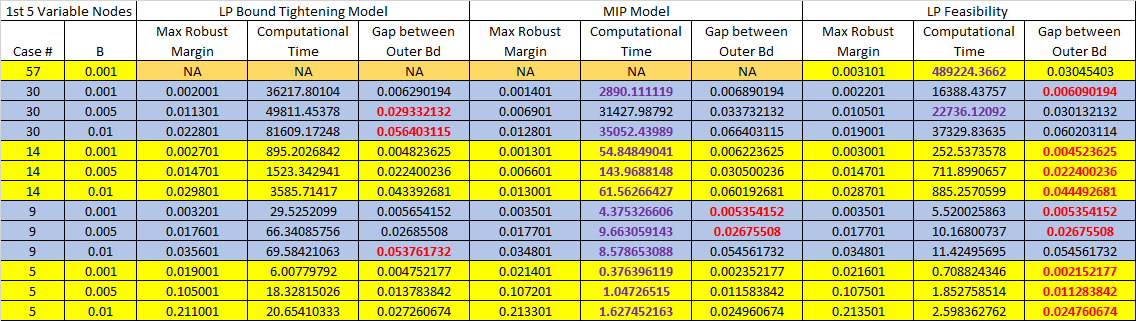
\includegraphics[scale=0.4]{Figures/InnerBoundTable} 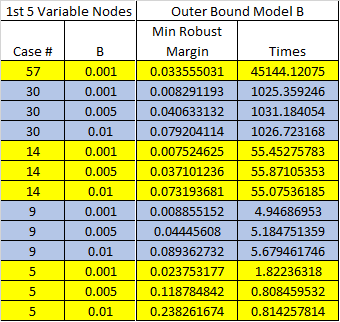
\includegraphics[scale=0.4]{Figures/OuterBoundTable} 
\end{center}
\label{tbl:Table1}
\end{figure} 
\begin{figure}[h]
\begin{center}
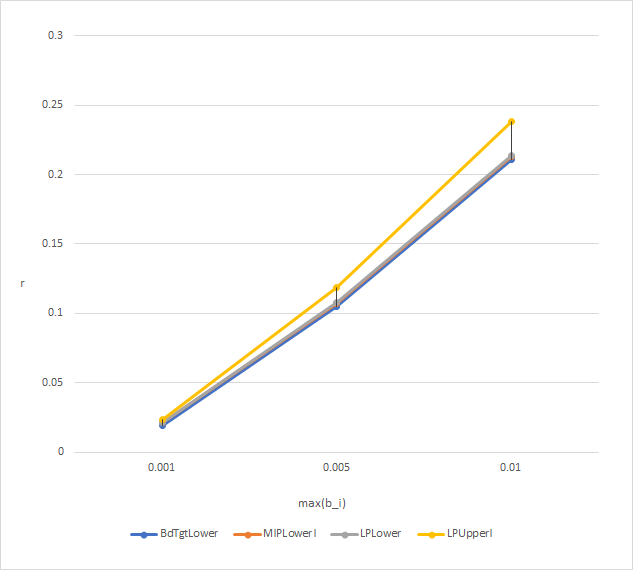
\includegraphics[scale=0.45]{Figures/Case5}
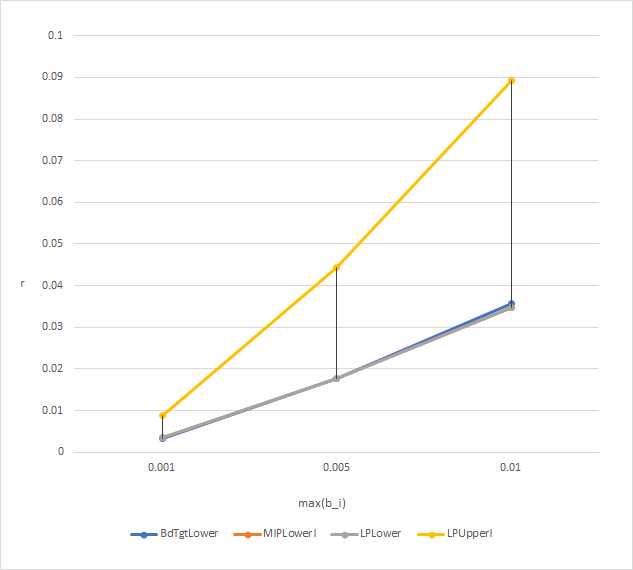
\includegraphics[scale=0.45]{Figures/Case9} \\
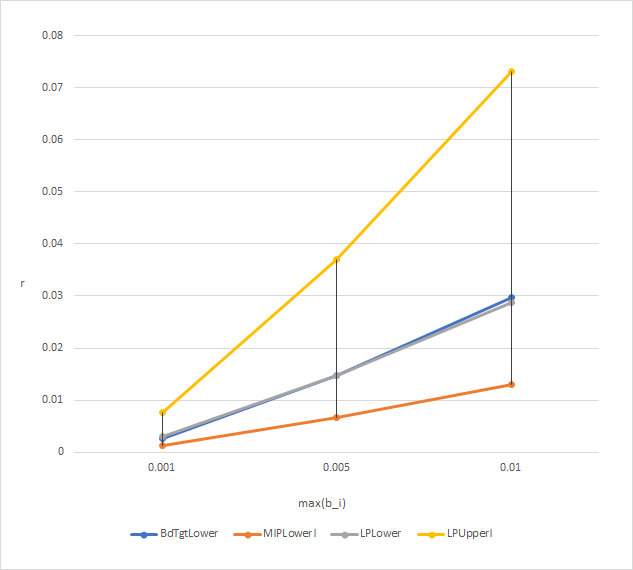
\includegraphics[scale=0.45]{Figures/Case14}
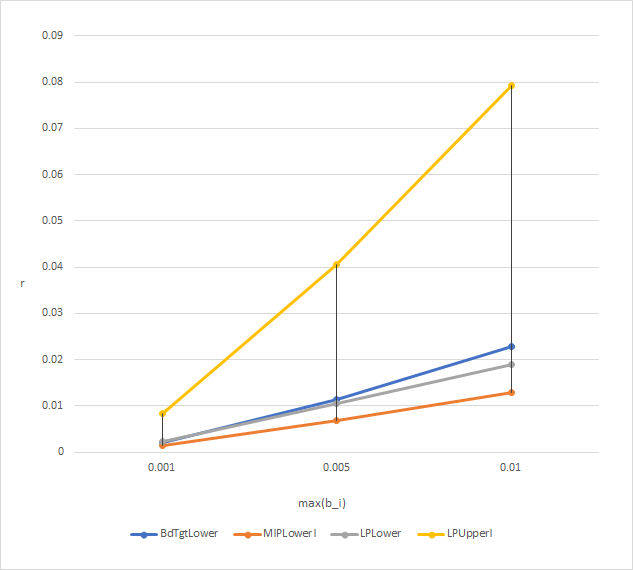
\includegraphics[scale=0.45]{Figures/Case30}
\caption{Case 5 (Top Left), Case 9 (Top Right), Case 14 (Bottom Left), Case 30 (Bottom Right)} \ \\
\end{center}
\label{fig:Graphs1}
\end{figure} 

The results are presented in table \ref{tbl:Table1} where each row of the table represents results conducted with $A\bold x\leq \bold b = B*ones$ for $B\in\{0.001, 0.005,0.01\}$ and $ones$ representing the vector of all ones of appropriate dimension. 
$A$ in this cases is a matrix s.t. $A\bold x\leq \bold b$ controls the flow between nodes in the power grid (i.e. each row of $A\bold x\leq \bold b$ has the form $x_i-x_j\leq b_k$. 
All computations were performed on a laptop running the 64bit Windows 10 operating system containing an Intel i-7 processor, 16 GB of Ram and 4 cores. 
Graphically we can look at this data on a case by case basis to highlight the effect of allowing more fluctuation between the nodes (i.e. as $B$ increases).(Figure \ref{fig:Graphs1}) 



%\begin{table}[h]
%\begin{center}
%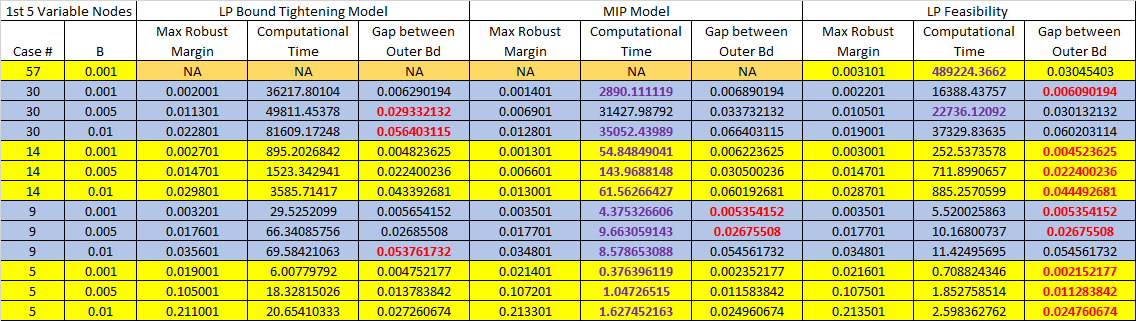
\includegraphics[scale=0.6]{Figures/InnerBoundTable}
%\caption{Robustness Margins for inner bound models } 
%\vspace{0.2in}
%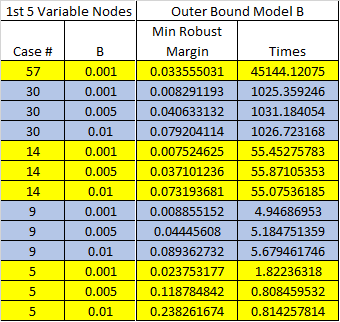
\includegraphics[scale=0.5]{Figures/OuterBoundTable}
%\caption{Robustness Margins for outer bound models}
%\end{center}
%\label{tbl:Table1}
%\end{table} 

As evident from table \ref{tbl:Table1} we have that the bound tightening model produces a better approximation of the inner bound on the robustness margin as the complexity of the data set increases. 
Certainly one would expect the bound tightening model to out perform the other inner bound models for all cases, but the choice of model parameters has a big effect on the efficiency of the model. 
For instance, setting a low tolerance for a minimal sufficient change in the dimensions of $\bold b$ will cause in most cases an extremely long running time. 
Thus in the extremely low and marginally high complexity cases it should be expected that the other models will out perform the bound tightening model as these manually set model parameters will have more of an impact on performance. 
Of special interest is the difference in performance of the MIP and Feasibility inner bound models as the complexity of the data increases. 
In particular it was surprising that the Feasibility model was the only inner bound model capable of efficiently computing the robustness margin for case 57 (see table \ref{tbl:Table1}). 
